Wie im Kapitel \ref{chap:quantile} gezeigt wurde, scheint sich die Abweichung im 99. Quantils des Niederschlags (und damit des Starkregens) nahezu unabhängig von den betreibenden Modellen (GCM und Re-Analysedaten) identisch abzuzeichnen. Die regionalen Klimamodelle bzw. deren Daten unterscheiden sich aber stark in der geographischen Ausbreitung der Abweichungen: Das Klimamodell mit parametrisierter Konvektion scheint über den gesamten Beobachtungsraum eine relativ gleichbleibende Abweichung zu erzeugen wohingegen das Klimamodell CCLM5-0-9 nur in gebirgigen Gegenden starke Abweichungen zeigt. Um nun kleiner Gebiete evaluieren zu können soll deshalb in diesem Kapitel wie es in \cite{biasMaraun} gemacht wurde, gezielt auf die Starkregenereignisse der unterschiedlichen Jahreszeiten eingegangen werden.
\section{Herangehensweise}\label{sec:Herangehensweise}
\begin{itemize}
\item Alle Datensätze werden auf die Jahreszeiten aufgeteilt:
	\subitem Frühling: 20. März - 20. Juni
	\subitem Sommer: 20. Juni - 22. September
	\subitem Herbst: 22. September - 21. Dezember
	\subitem Winter: 21. Dezember - 20. März
\item Von diesen neu aufgeteilten Datensätzen werden die 99. Quantile berechnet
\item Diese Quantile werden mit den Beobachtungsdaten verglichen.
\end{itemize}

\section{Differenzen in den Jahreszeiten}
Es wurde wie im Unterkapitel \ref{sec:Herangehensweise} erklärt, die Daten zunächst auf die Jahreszeiten aufgeteilt und dann daraus (über alle zehn Jahre) die maximalen Niederschläge herausgefiltert - über die Berechnung des 99. Quantils. Danach wurde, wie schon in den Kapiteln zuvor beschrieben von den Modelldaten die Beobachtungsdaten abgezogen- das heißt, wenn die Differenz negativ ist wurde zu wenig Niederschlagsmenge modelliert und vice versa.\\
Aus diesen Abweichungen wurden die Boxplots in Abb.\ref{fig:seasons_boxplots} erstellt: Alle Abweichungen scheinen sich in einem relativ guten Rahmen aufzuhalten. Nur der Evaluation-Datensatz aus ALP-3 scheint enorme Ausreißer zu haben. Dies ist wiederum auf das Gebiet im Süden Kroatiens zurückzuführen, wie in der Abbildung \ref{fig:seasons_dif} zu erkennen ist. In der Tabelle \ref{tab:season_bias} wurde die schlechteste Performance nach der Jahreszeit der Datensätze eingetragen. Da hier nur drei von zwei Datensätzen auftauchten, wurde noch eine zweite Tabelle angelegt, die die schlechteste Jahreszeit für jeden Datensatzes darstellt. Diese ist in Tabelle \ref{tab:season_dataset} untergebracht. Die Einträge der Tabelle\ref{tab:season_dataset} und der Tabelle\ref{tab:season_bias} wurden dann verwendet, um über die Datensätze der Folgenden näheren Betrachtungen zu entscheiden:
\begin{itemize}
	\item Für den Datensatz Historical EUR-11: Frühling
	\item Für den Datensatz Evaluation EUR-11: Sommer
	\item Für den Datensatz Historical ALP-3: Sommer
	\item Für den Datensatz Evaluation ALP-3: Frühling
\end{itemize}
Dadurch konnten die Datensätze für dasselbe Phänomen auch untereinander verglichen werden. Auch wenn dies bedeutet, dass Winter und Herbst nicht weiter genauer betrachtet werden. Jedoch ist in Abb.\ref {fig:seasons_boxplots} zu erkennen dass sich die Abweichungen dieser beiden Jahreszeiten ähnlich wie im Frühling verhalten.
\begin{table}[h]
	\begin{tabularx}{\textwidth}{|X|X|X|X|}
		\hline
		\textbf{Frühling} & \textbf{Sommer}& \textbf{Herbst} & \textbf{Winter}\\
		\hline
		\textbf{Evaluation ALP-3}  & \textbf{Historical ALP-3}  & \textbf{Evaluation EUR-11} & \textbf{Historical ALP-3} \\
		Bias:$7.01032\frac{mm}{Tag}$& Bias:$6.68616\frac{mm}{Tag}$ & Bias: $-4.28896\frac{mm}{Tag}$ & Bias:$8.33802\frac{mm}{Tag}$\\
		\hline
	\end{tabularx}
	\caption{Schlechteste Performance nach Extremniederschlägen in den Jahreszeiten gemessen am Bias}
	\label{tab:season_bias}
\end{table}
\begin{table}[h]
	\begin{tabularx}{\textwidth}{|X|X|X|X|}
		\hline
		\textbf{Historical EUR-11} & \textbf{Evaluation EUR-11}& \textbf{Historical ALP-3} & \textbf{Evaluation ALP-3}\\
		\hline
		\textbf{Frühling}  & \textbf{Sommer}  & \textbf{Winter} & \textbf{Frühling} \\
		Bias:$5.36773\frac{mm}{Tag}$& Bias:$5.33069\frac{mm}{Tag}$ & Bias:$8.33802\frac{mm}{Tag}$ & Bias:$7.01032\frac{mm}{Tag}$\\
		\hline
	\end{tabularx}
	\caption{Schlechteste Performance der einzelnen Datensätze nach Extremniederschlägen in den Jahreszeiten gemessen am Bias}
	\label{tab:season_dataset}
\end{table}
\begin{figure}
	\begin{subfigure}{0.49\textwidth}
		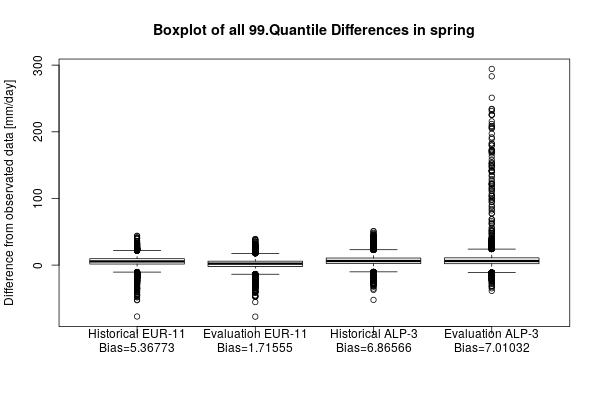
\includegraphics[width=\textwidth]{quantile_season/boxplot_spring.jpg}
		\caption{Frühling}
	\end{subfigure}
	\begin{subfigure}{0.49\textwidth}
		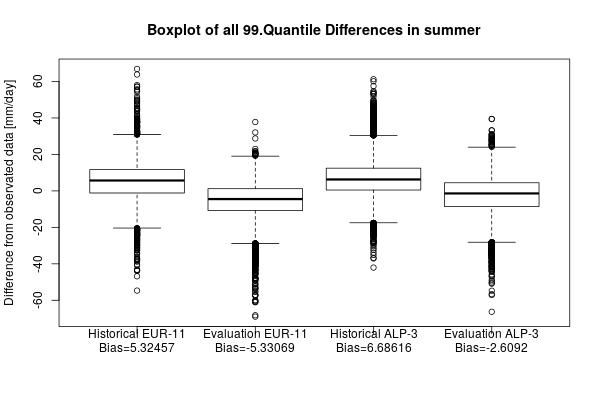
\includegraphics[width=\textwidth]{quantile_season/boxplot_summer.jpg}
		\caption{Sommer}
	\end{subfigure}
	\begin{subfigure}{0.49\textwidth}
		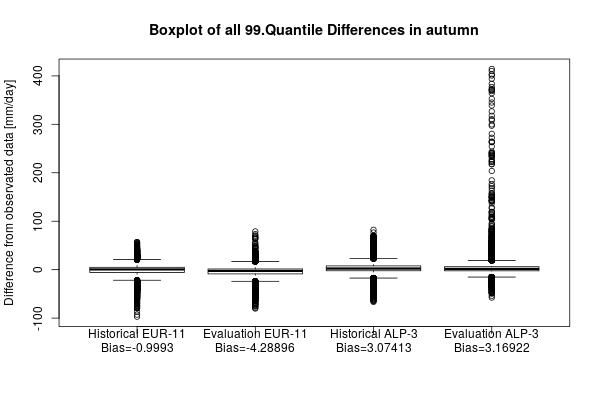
\includegraphics[width=\textwidth]{quantile_season/boxplot_autumn.jpg}
		\caption{Herbst}
	\end{subfigure}
	\begin{subfigure}{0.49\textwidth}
		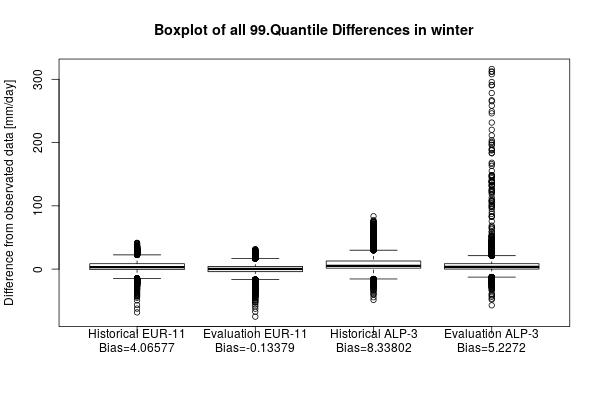
\includegraphics[width=\textwidth]{quantile_season/boxplot_winter.jpg}
		\caption{Winter}
	\end{subfigure}
	\caption{Boxplots der Starkniederschläge in den verschiedenen Jahreszeiten}
	\label{fig:seasons_boxplots}
\end{figure}
\begin{figure}
	\begin{subfigure}{0.49\textwidth}
		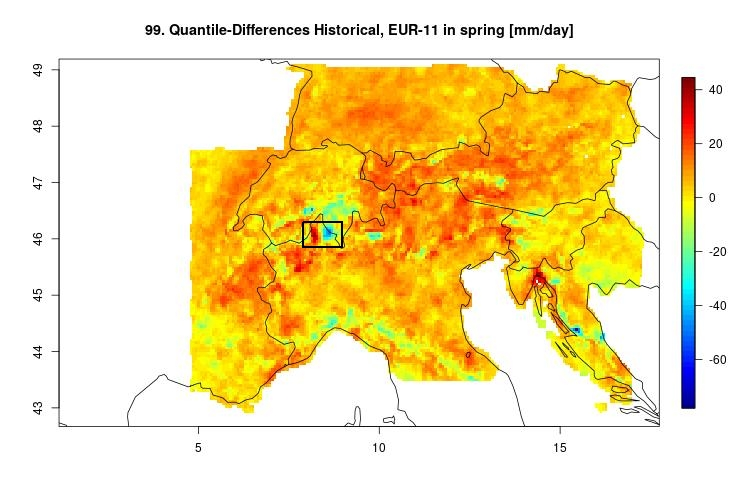
\includegraphics[width=\textwidth]{quantile_season/hist_eur11_spring.jpg}
		\caption{Historical, EUR-11 Frühling}
		\label{fig:seasons_dif:hist_eur11}
	\end{subfigure}
	\begin{subfigure}{0.49\textwidth}
		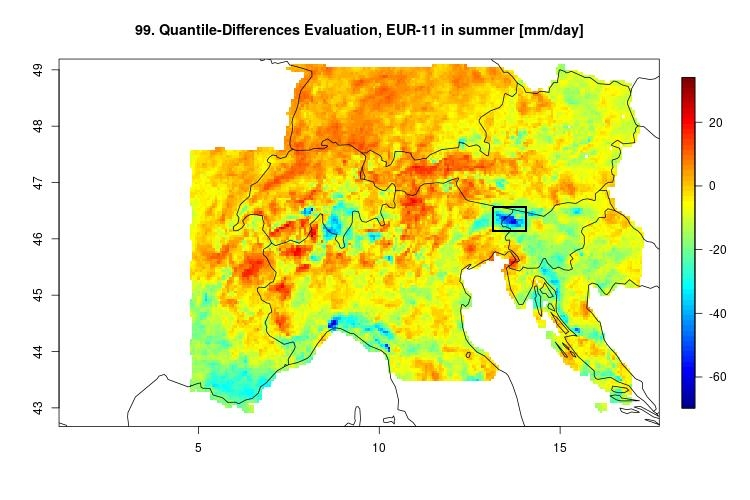
\includegraphics[width=\textwidth]{quantile_season/eval_eur11_summer.jpg}
		\caption{Evaluation, EUR-11, Sommer}
		\label{fig:seasons_dif:eval_eur_11}
	\end{subfigure}
	\begin{subfigure}{0.49\textwidth}
		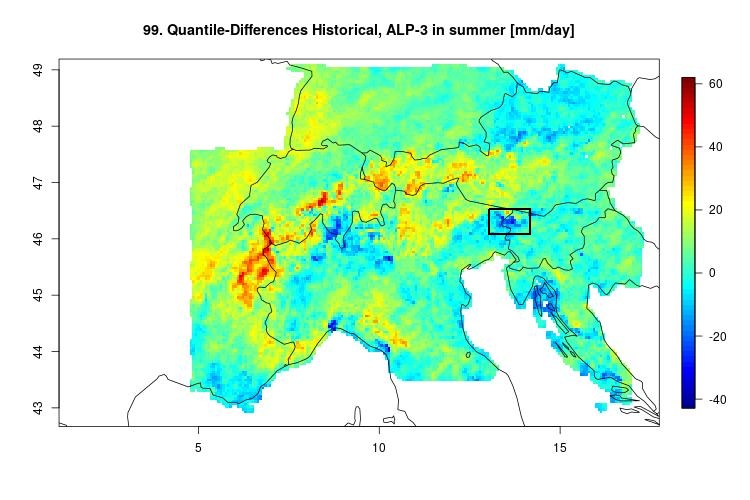
\includegraphics[width=\textwidth]{quantile_season/hist_alp3_summer.jpg}
		\caption{Historical, ALP-3 Sommer}
		\label{fig:seasons_dif:hist_alp3}
	\end{subfigure}
	\begin{subfigure}{0.49\textwidth}
		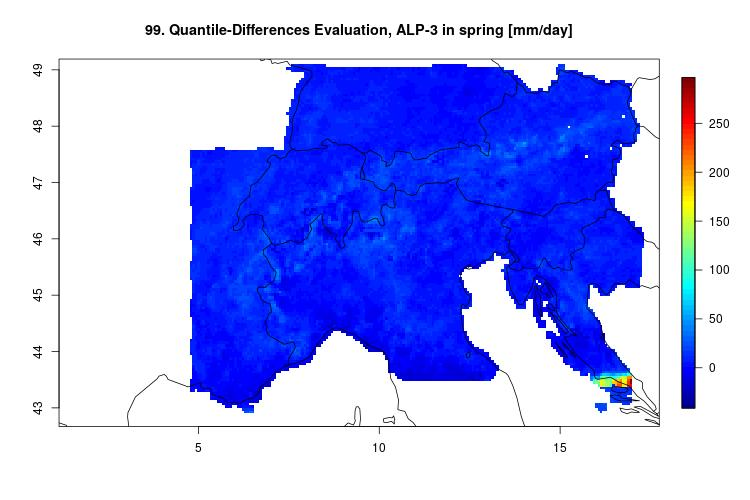
\includegraphics[width=\textwidth]{quantile_season/eval_alp3_spring.jpg}
		\caption{Evaluation, ALP-3 Frühling}
	\end{subfigure}
	\caption{Differenzen der in der Tabelle \ref{tab:season_dataset} angeführten Testfälle mit gekennzeichneten Bereichen}
	\label{fig:seasons_dif}
\end{figure} \newpage
\section{Nähere Betrachtungen der einzelnen Datensätze}
\subsection{Historical EUR-11} \label{subsec:hist_eur11}
Wie man in der Abbildung \ref{fig:seasons_dif:hist_eur11} erkennen kann, liegen in dem gekennzeichneten Bereichen die maximalen negativen Abweichungen direkt neben denen der maximal Positiven. Dieses Phänomen scheint mehrmals auf der Karte aufzutauchen (z.B im Bereich von Krk und im Bereich der Alpi Orobie). Dies lässt darauf schließen, dass das Modell eine große Regenzelle aufgrund von Fehlberechnungen örtlich Fehlerhaft abbildete. Diese Vermutung kann gut durch die in Abb. \ref{fig:seasons_hist} dargestellten Niederschlagskarten nachvollzogen werden. Jedoch ist Bemerkenswert, dass das Modell solch starke Abweichungen aus dem Normalzustand überhaupt abbildet: Die Peaks, die diese Abweichungen ausmachen liegen weit über dem Durchschnitt dieser Regionen vgl. dazu Abb.\ref{fig:season:over_apgd} \& \ref{fig:season:under_apgd}.\\
Um dieses Phänomen näher zu erkunden wurde der gekennzeichneten Bereich in einen überschätzenden und einen unterschätzenden Bereich geteilt. Die Modelldaten wurden dann im Frühling über die Fläche gemittelt und in Abb.\ref{fig:season:over_hist} \& \ref{fig:season:under_hist} gegen die Zeit aufgetragen. Dieselben Berechnungen im selben Bereich wurden für die Beobachtungsdaten vollzogen. Diese Ergebnisse wurden in der Abb.\ref{fig:season:under_apgd} \& \ref{fig:season:over_apgd} visualisiert.\\
\begin{figure}[h]
	\begin{subfigure}{0.49\textwidth}
		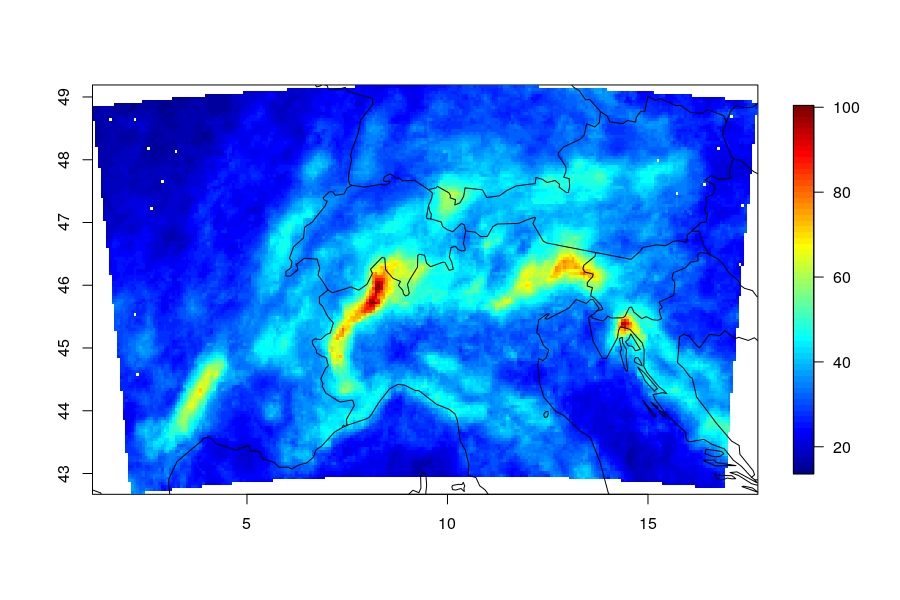
\includegraphics[width=\textwidth]{quantile_season/hist_eur_11_clean.jpg}
		\caption{Historical, EUR-11}
		\label{fig:seasons_hist:hist}
	\end{subfigure}
	\begin{subfigure}{0.49\textwidth}
		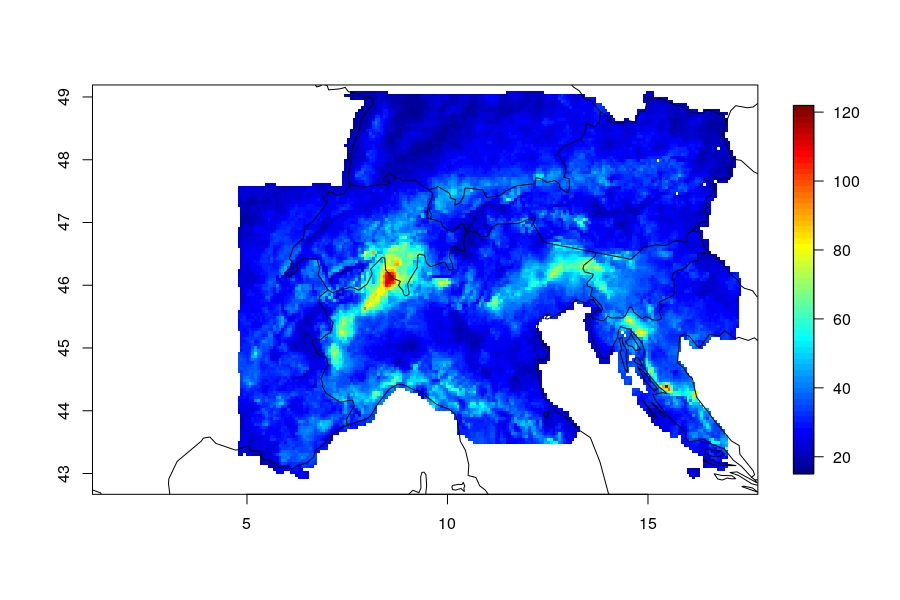
\includegraphics[width=\textwidth]{quantile_season/apgd_spring.jpg}
		\caption{APGD}
		\label{fig:seasons_hist:apgd}
	\end{subfigure}
	\caption{Die 99. Quantile der Datensätze EUR-11 und APGD für den Frühling}
	\label{fig:seasons_hist}
\end{figure}
\begin{figure}[h]
	\begin{subfigure}{0.49\textwidth}
		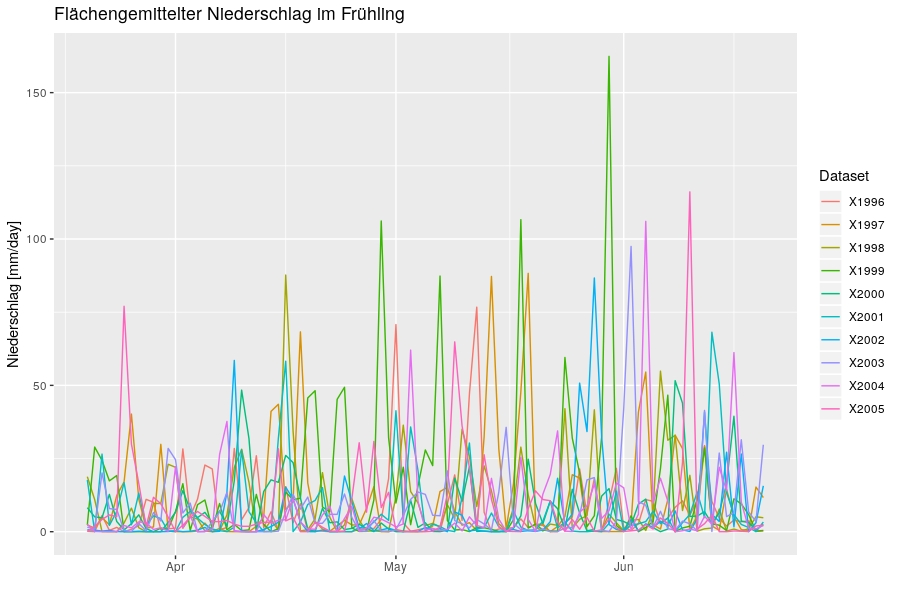
\includegraphics[width=0.95\textwidth]{quantile_season/hist_eur11_oversim1.jpeg}
		\caption{Überschätzender Bereich}
		\label{fig:season:over_hist}
	\end{subfigure}
	\begin{subfigure}{0.49\textwidth}
	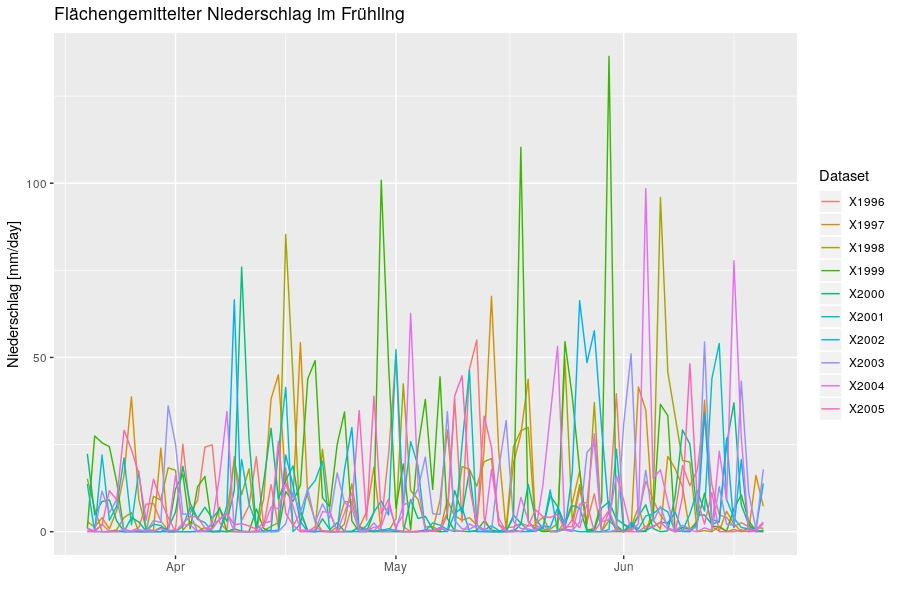
\includegraphics[width=0.95\textwidth]{quantile_season/hist_eur11_undersim1.jpeg}
	\caption{Unterschätzender Bereich}
	\label{fig:season:under_hist}
	\end{subfigure}
	\caption{Gemittelte Niederschlagsmenge im entsprechenden Bereich (vgl. Abb.\ref{fig:seasons_dif:hist_eur11}) des Datensatzes Historical, EUR-11}
\end{figure}
\begin{figure}[h]
	\begin{subfigure}{0.49\textwidth}
		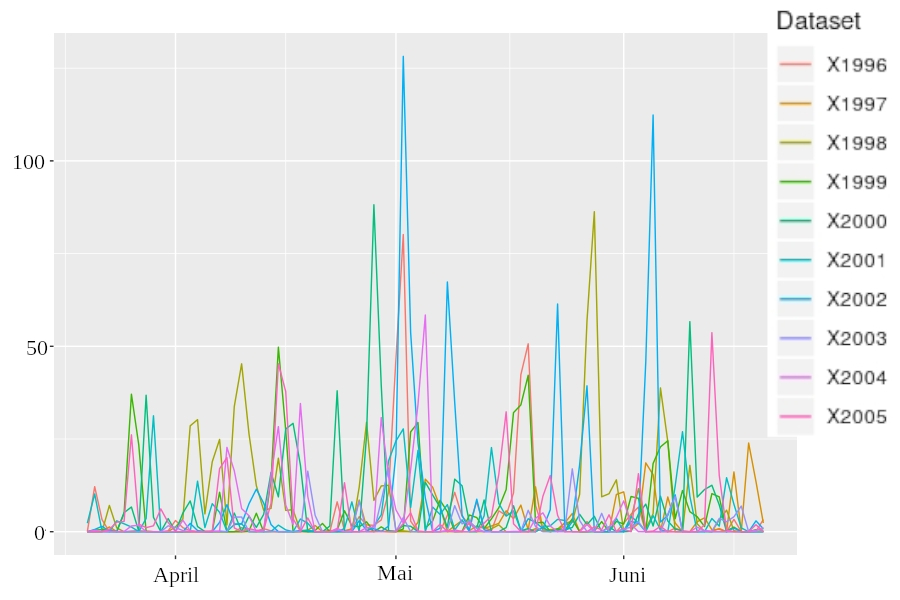
\includegraphics[width=0.95\textwidth]{quantile_season/apgd_oversim1.jpeg}
		\caption{Überschätzender Bereich}
		\label{fig:season:over_apgd}
	\end{subfigure}
	\begin{subfigure}{0.49\textwidth}
		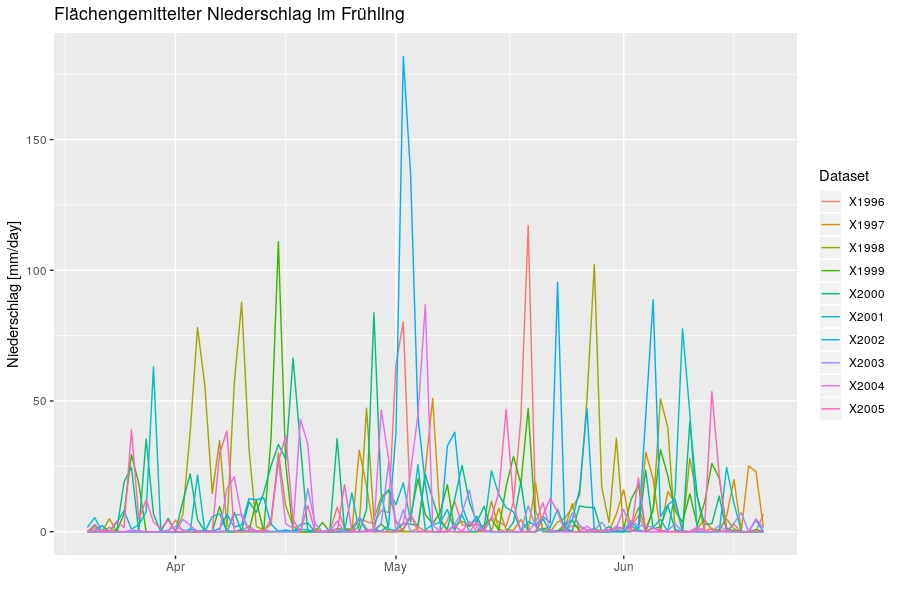
\includegraphics[width=0.95\textwidth]{quantile_season/apgd_undersim1.jpeg}
		\caption{Unterschätzender Bereich}
	\label{fig:season:under_apgd}
	\end{subfigure}
	\caption{Gemittelte Niederschlagsmenge im entsprechenden Bereich (vgl. Abb \ref{fig:seasons_dif:hist_eur11}) der Beobachtungsdaten}
\end{figure}

Um nun das Phänomen, welches die extreme Abweichung verursacht hat, genauer zu betrachten wurden von den beiden Plots ein Jahr ausgewählt, welches augenscheinlich die Abweichung verursacht:
\begin{itemize}
	\item Überschätzender Bereich: Im Jahr 1999 sagt das Modell den größten Peak voraus, welcher in den Beobachtungsdaten nicht zu finden ist.
	\item Unterschätzender Bereich: Im Jahr 2000 wurde die größte Niederschlagsmenge im Frühling beobachtet, diese ist wiederum nicht in den Modelldaten zu finden
\end{itemize}
Für diese beiden Jahre wurde in der gemittelten Fläche der Niederschlag zum Durchschnitt des Niederschlags aufgezeichnet. Das Ergebnis ist in der Abbildung \ref{fig:seasons:hist_eur11:overundersim_mean} dargestellt.\\

\begin{figure}[h]
	\begin{subfigure}{0.49\textwidth}
		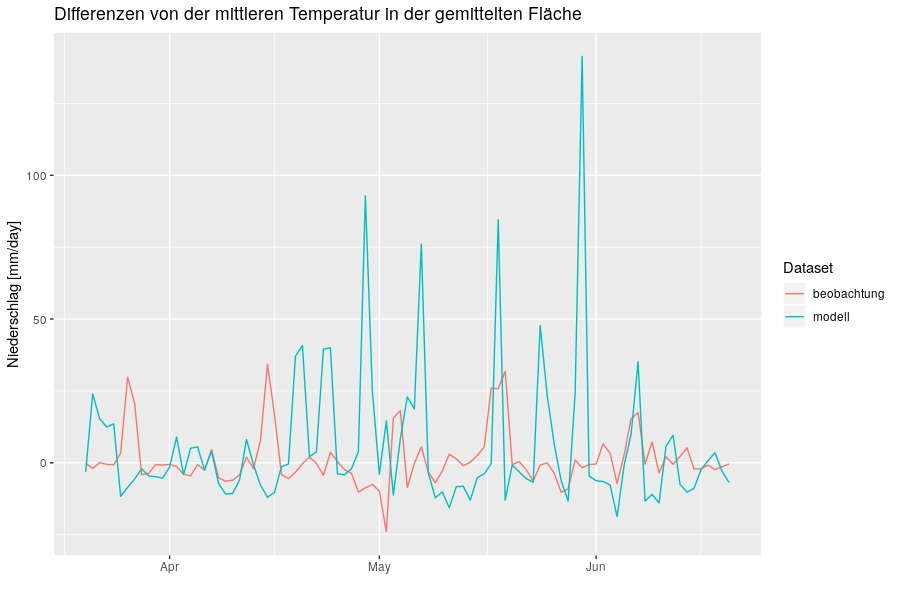
\includegraphics[width=\textwidth]{quantile_season/hist_eur11_oversim_mean.jpeg}
		\caption{überschätzender Bereich, Jahr 1999, Frühling}
		\label{fig:seasons:hist_eur11:oversim_mean}
	\end{subfigure}
	\begin{subfigure}{0.49\textwidth}
		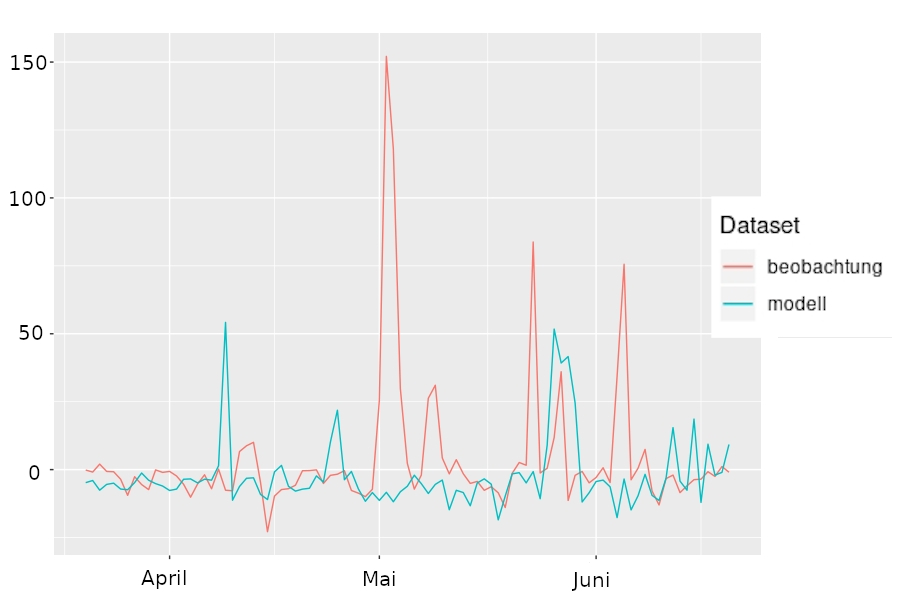
\includegraphics[width=\textwidth]{quantile_season/hist_eur11_undersim_mean.jpeg}
		\caption{unterschätzender Bereich, Jahr 2000, Frühling}
		\label{fig:seasons:hist_eur11:undersim_mean}
	\end{subfigure}
	\caption{Abweichung vom mittleren Niederschlag im entsprechenden Bereich, Modelldaten= Historical EUR-11}
	\label{fig:seasons:hist_eur11:overundersim_mean}
\end{figure}
Man erkennt gut, dass im überschätzendem Bereich Abb.\ref{fig:seasons:hist_eur11:oversim_mean} die Modelldaten eine viel stärker fluktuierende Kurve, mit größeren Ausschlägen hat als die Beobachtungsdaten.
Im unterschätzenden Bereich (Abb.\ref{fig:seasons:hist_eur11:undersim_mean}) gilt dasselbe: Es gleicht der Kurvenverlauf des Modells im unterschätzendem Bereich der Kurve der Beobachtungsdaten im überschätzendem Bereich und vice versa.\newpage

\subsection{Evaluation EUR-11}\label{sec:eval_eur_11}
In diesem Datensatz fällt auf, dass mehrere große Bereiche vom Modell unterschätzt wurden. Dies zeigt sich besonders gut in den ausgeprägten blauen Flecken der Abb.\ref{fig:seasons_dif:eval_eur_11}. Es treten kaum so starke Überschätzungen wie beim Historical Datensatz auf. Dies könnte auch an der betrachteten Jahreszeit liegen: Sommer ist die Heimat der Hitzegewitter und somit auch der kurzzeitigen Extremniederschläge, welche eine große Herausforderung in der Simulation sind. Besonders wenn die Konvektion parametrisiert wurde, wie es in diesem Modell der Fall ist. Aufgrund der Jahreszeit wird für diesen Datensatz die Temperatur und der Niederschlag in dem gekennzeichneten Bereich mit den Beobachtungsdaten verglichen.\\
Wie man in der Abbildung \ref{fig:season:under_eval_eur11} erkennt, ist der Niederschlag in einer für parametrisierte Konvektion typische Fluktuation nahezu gleichmäßig über die Zeit verteilt. Es gibt keine großen Ausreißer. Dies fällt besonders auf, wenn man das Mittel der Beobachtungsdaten damit vergleicht (Abb.\ref{fig:season:under_apgd_eur11}). Des Weiteren kann man dem Diagramm der Beobachtungsdaten entnehmen, dass sich der ausschlaggebende Peak im September 1998 befindet, Für diese Zeit herrscht in diesem Gebiet eine Differenz von ungefähr $-60\frac{mm}{Tag}$. Der beobachtete Niederschlag im September dieses Jahres schien besonders heftig auszufallen. was durch die Kurve des Modells kaum abgebildet wird - dort herrscht ein monotones fluktuieren des Niederschlags ohne größere Ausreißer.\\
Um nun die Temperatur in Verbindung mit der starken Abweichung des Niederschlags zu bringen und um eventuell auch ein untypisches Wetterverhalten in diesem Jahr auszumachen wurde die Temperaturkarte für dieses Gebiet ausgeschnitten und, dem Niederschlag gleich, über die Fläche gemittelt.\\
Der Niederschlag und die Temperatur wurden im Jahr 1998 betrachtet: Der Kurvenverlauf des Niederschlags in der Abbildung \ref{fig:seasons:undersim_eval_eur11} zeigt eine gute Übereinstimmung zwischen Modell und Beobachtungen: Einzig der Ausschlag der Kurven ist etwas zu klein, was für die Vorhersagekraft eines Modells mit parametrisierter Konvektion spricht. Es kann zwar ein den Beobachtungen ähnlicher Verlauf der Temperaturkurven beobachtet werden, jedoch scheint diese nicht den tatsächlichen Werten nahezukommen und fluktuiert eher in einer ähnlichen Frequenz. Da es sich hier um eine rein qualitative Analyse handelt dürfen nicht Werte aus den Vergleichen gezogen werden sondern nur auf das ähnliche oder unähnliche Verhalten des Modells zu den Beobachtungsdaten geschlossen werden.

\begin{figure}[h]
	\begin{subfigure}{0.49\textwidth}
		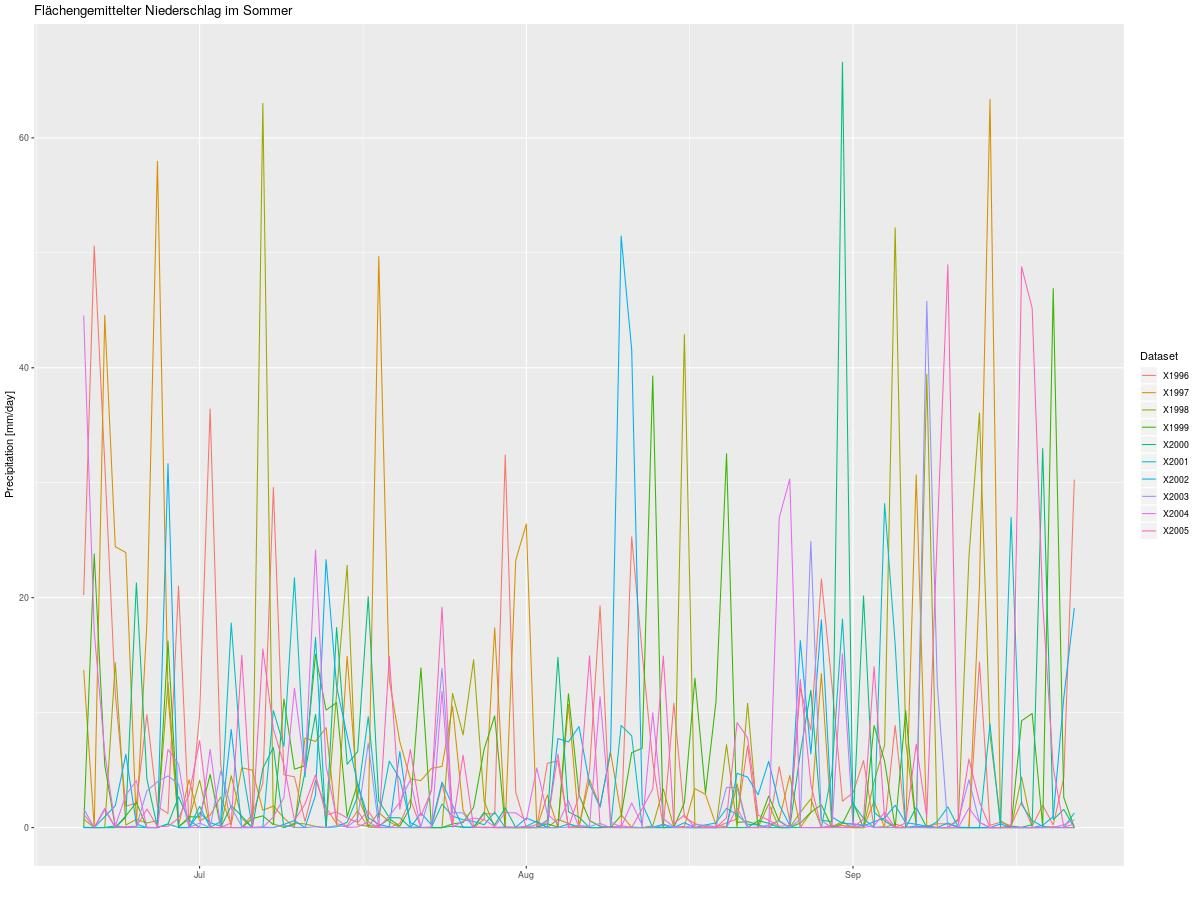
\includegraphics[width=\textwidth]{quantile_season/eval_eur11_undersim.jpg}
		\caption{Flächenmittel des Niederschlags im unterschätzenden Gebiet, gekennzeichnet in Abb.\ref{fig:seasons_dif:hist_eur11} für den Datensatz Evaluation, EUR-11}
		\label{fig:season:under_eval_eur11}
	\end{subfigure}
	\begin{subfigure}{0.49\textwidth}
		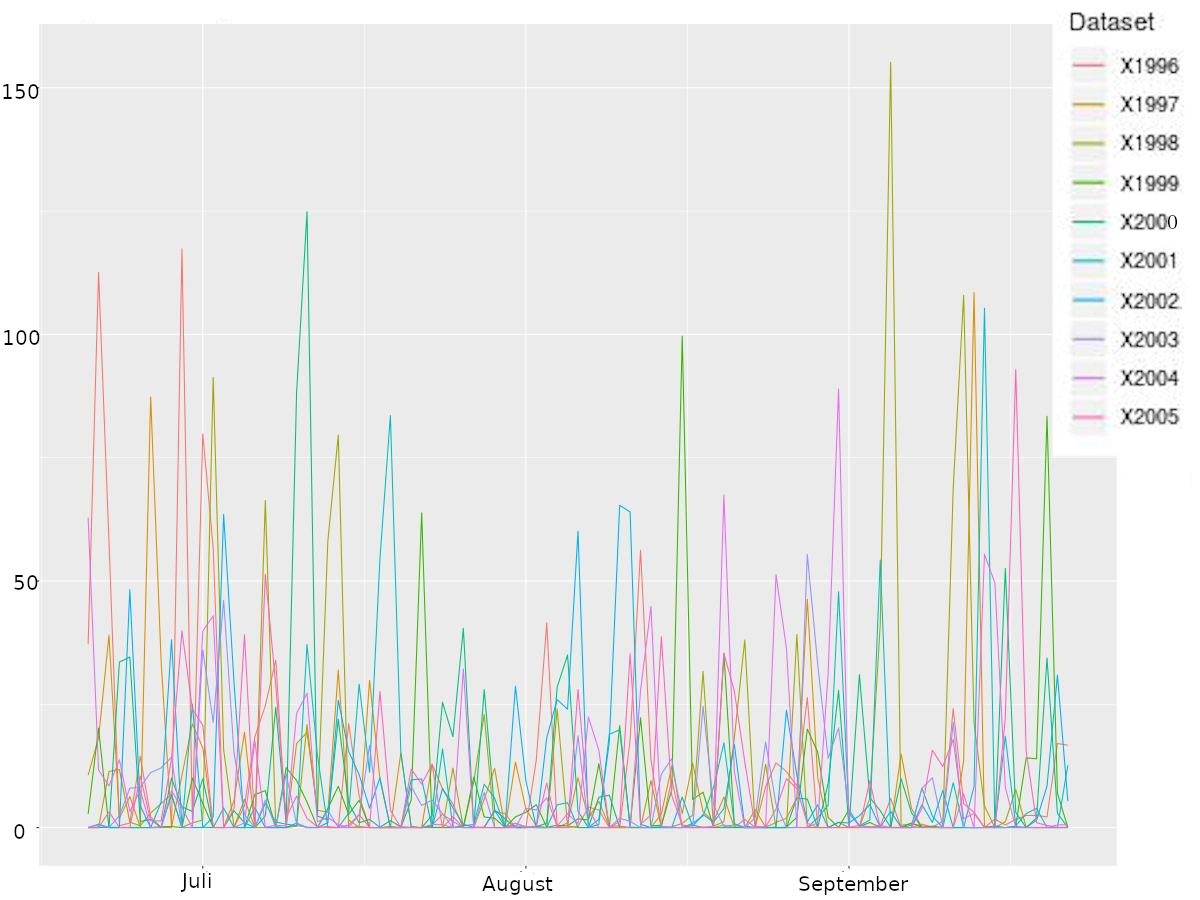
\includegraphics[width=\textwidth]{quantile_season/apgd_undersim_eur11.jpg}
		\caption{Flächenmittel des Niederschlags im unterschätzenden Gebiet, gekennzeichnet in Abb.\ref{fig:seasons_dif:hist_eur11} für den Beobachtungs-Datensatz APGD}
		\label{fig:season:under_apgd_eur11}
	\end{subfigure}
	\caption{}
\end{figure}

\begin{figure}[h]
	\begin{subfigure}{0.49\textwidth}
		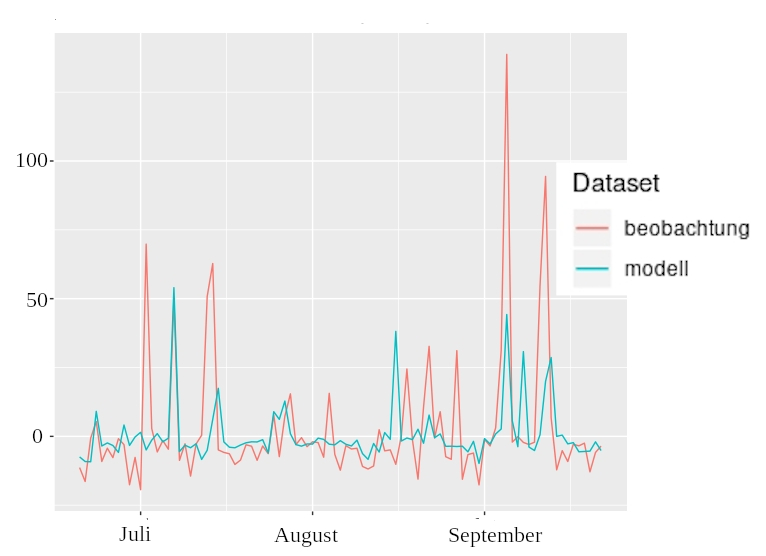
\includegraphics[width=\textwidth]{quantile_season/middle_pr_undersim_eur11.jpg}
		\caption{Niederschlag}
	\end{subfigure}
	\begin{subfigure}{0.49\textwidth}
		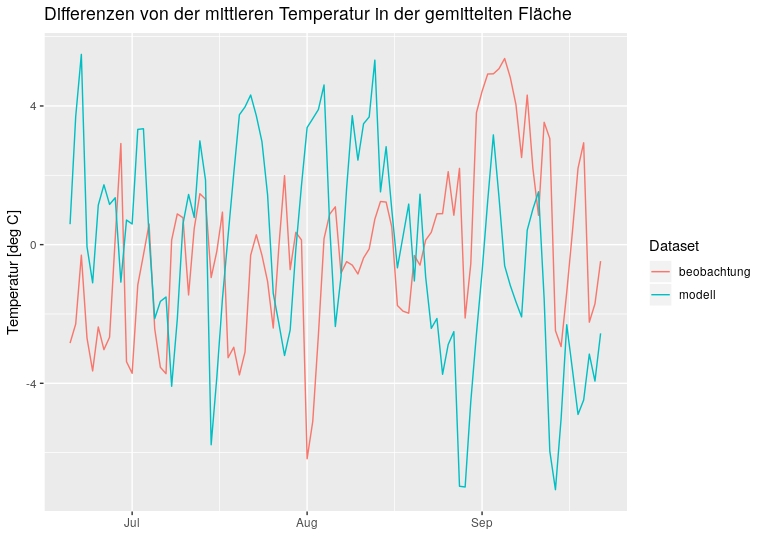
\includegraphics[width=\textwidth]{quantile_season/middle_temp_undersim_eur11.jpg}
		\caption{Temperatur}
	\end{subfigure}
	\caption{Differenz der Temperatur und des Niederschlags zum Durchschnitt (Evaluation EUR-11 Jahr 1998) in der in Abb.\ref{fig:seasons_dif:eval_eur_11} gekennzeichneten Fläche}
	\label{fig:seasons:undersim_eval_eur11}
\end{figure}

\begin{itemize}
	\item Der Niederschlag liegt im Monat September über dem Durchschnittsniederschlag. Dies gilt für Modell und Beobachtungsdaten, was eine gute Vorhersagekraft des Modells verspricht. Beachtenswert dabei ist, dass der Niederschlag im Modell über die ganze Zeitspanne viel weniger vom Mittelwert abweicht als es in den Beobachtungsdaten der Fall ist.
	\item Die betreffende Temperaturkurve ist viel weniger stark korrelierend. Im Monat September, wo die Starkregenereignisse dieses Gebiets häufiger auftreten, scheinen die Modelldaten eine auf den Durchschnitt bezogene kältere Temperatur vorherzusagen. Das könnte auch auf einen Fehler in den Re-Analysedaten hinweisen.
\end{itemize}
\newpage

\subsection{Historical ALP-3}
Wie in der Abbildung \ref{fig:seasons_dif:hist_alp3} zu sehen ist, wird in diesem Kapitel derselbe Bereich evaluiert, wie bereits im zuvor im Kapitel \ref{sec:eval_eur_11}. Dadurch können die beiden Modelle und auch die Antriebsdaten gegeneinander verglichen werden. Da das Modell CCLM5-0-9 im ALP-3 Historical Datensatz mit historischen Daten des globalen Klimamodells MPI-ESM-LR angetrieben, dadurch sollten theoretisch größere Abweichungen herrschen als in dem mit Re-Analysedaten betriebenen.\\
Wieder wurden wie im Kapitel zuvor schon die Daten über die in Abb.\ref{fig:seasons_dif:hist_alp3} gekennzeichnete Fläche gemittelt und mit den Beobachtungsdaten verglichen, da in demselben Bereich eine relativ große negative Abweichung vorzufinden war. Dabei blieb natürlich der Beobachtungsdatensatz derselbe und es wird deshalb darauf verzichtet, den Plot in Abb.\ref{fig:season:under_apgd_eur11} nochmal abzubilden. Die Modelldaten sind in der Abb.\ref{fig:season:under_hist_alp3}\\
Man erkennt, dass sich das Muster für den Niederschlag kaum verändert hat. Der Zusammenhang mit den Beobachtungsdaten hat sich sogar etwas verschlechtert: Da die Übereinstimmung des Peaks im September überhaupt nicht mehr gegeben ist. Auch beim Betrachten der Abb.\ref{fig:season:under_hist_alp3} fällt dies bereits auf. Da das regionale Modell in das gröber aufgelöste CCLM4-8-17 eingenestet wurde, kann diese Verschlechterung der Korrelation auch auf das Aufschaukeln der Fehler beider Modelle zurückgeführt werden.\\
Die Temperatur scheint jedoch um einiges besser den Gegebenheiten zu entsprechen, die Fluktuationen über und unter der Durchschnittstemperatur entsprechen nahezu perfekt denen in den Beobachtungsdaten. Somit kann für das Konvektion-Erlaubende Klimamodell CCLM5-0-9 gesagt werden, dass die Temperaturfluktuationen im Sommer um einiges besser dargestellt werden.
\begin{figure}[h!]
	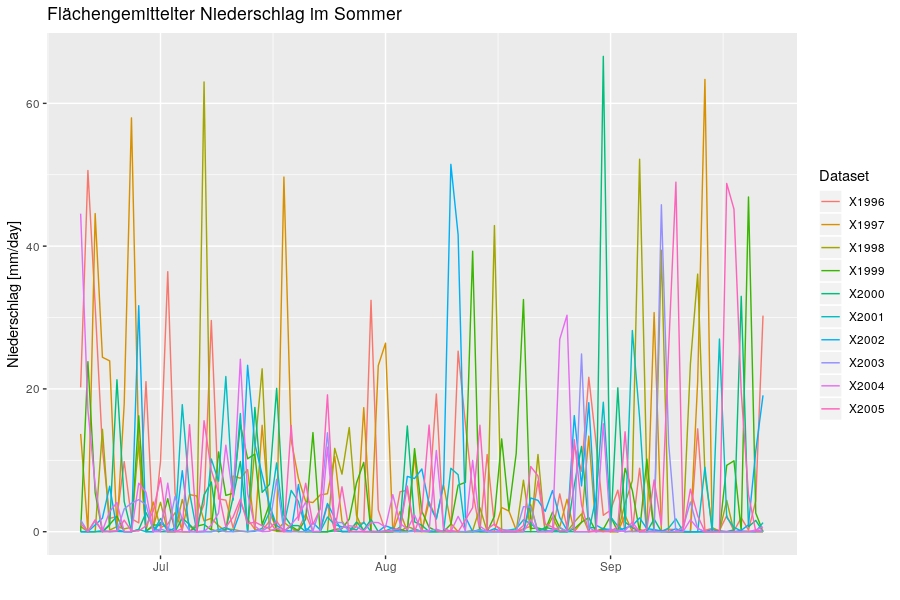
\includegraphics[width=0.95\textwidth]{quantile_season/hist_alp3_undersim.jpg}
	\caption{Niederschlagsverlauf im Datensatz Historical, ALP-3 für den in Abb.\ref{fig:seasons_dif:hist_alp3} gekennzeichneten Bereich, gemittelt über dessen Fläche}
	\label{fig:season:under_hist_alp3}
\end{figure}
\begin{figure}[h!]
	\begin{subfigure}{0.49\textwidth}
		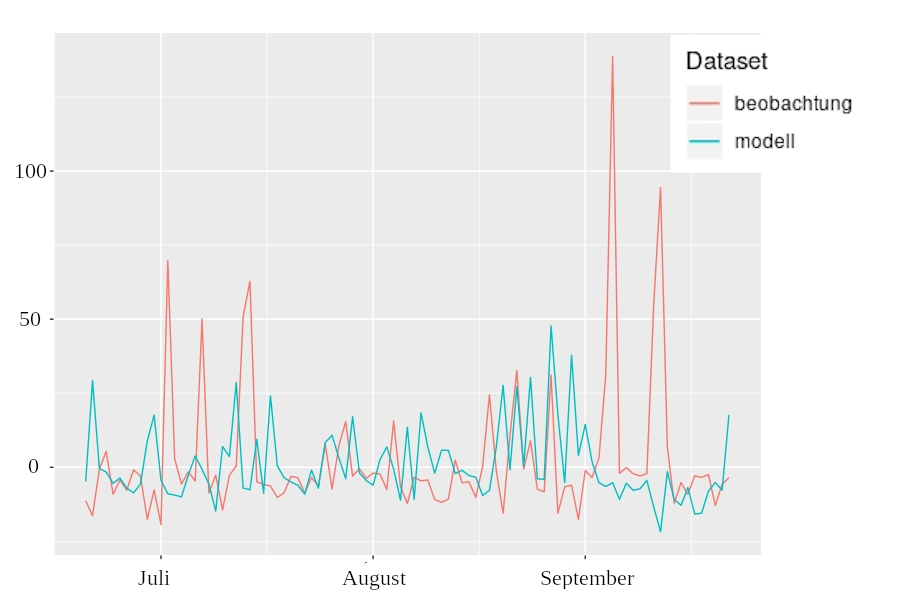
\includegraphics[width=\textwidth]{quantile_season/dif_pr_undersim_alp3.jpeg}
		\caption{Niederschlag}
	\end{subfigure}
	\begin{subfigure}{0.49\textwidth}
		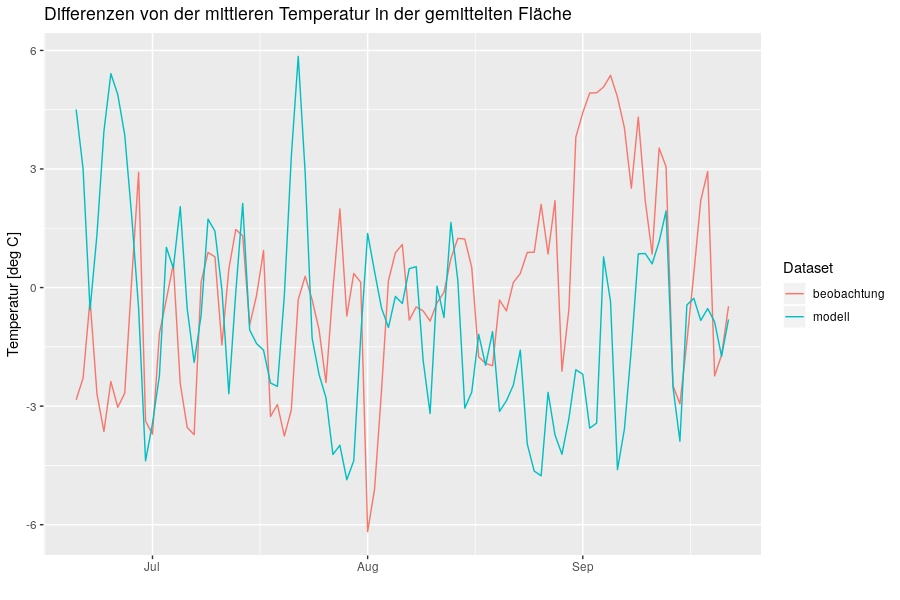
\includegraphics[width=\textwidth]{quantile_season/dif_temp_undersim_alp3.jpeg}
		\caption{Temperatur}
	\end{subfigure}
	\caption{Differenz der Temperatur und des Niederschlags zum entsprechenden Durchschnitt. Modelldaten: Historical ALP-3, in der in Abb.\ref{fig:seasons_dif:hist_alp3} gekennzeichneten Fläche (im Jahr 1998)}
	\label{fig:seasons:mean_alp3}
\end{figure}

\newpage
\subsection{Evaluation ALP-3}\label{subsec:eval_alp3}
Um den Datensatz Evaluation ALP-3 mit dessen größten Abweichungen besser darstellen zu können, wurde zunächst das Gebiet im Süden Kroatiens ausgeschnitten und verworfen, um dessen Verfälschung auszublenden. Diese Abweichung kann durch die Einwirkung der Randbedingungen und die damit verbundenen Probleme des globalen Modells auf das RCM erklärt werden(in Kapitel \ref{sec:problems_in_simulation} genauer beschrieben). Die Karte des Niederschlags, die sich daraus ergab findet man in Abb.\ref{fig:seasons:cropped eval_alp_3}. Wie zu erkennen ist, hat sich die höchste Niederschlagsdifferenz von $250\frac{mm}{Tag}$ auf etwa $60\frac{mm}{Tag}$ vermindert - dieses Gebiet scheint eine Fehlsimulation durch Interpolation am Rande des Darstellungsbereiches zu sein. Der Boxplots in Abb.\ref{fig:seasons:cropped eval_alp_3_boxplot} unterstützt diese Vermutung: der Bias hat sich drastisch verkleinert: von anfänglich $7.01032$ auf $4.95719$. Durch diese verbesserte Darstellung wurde ersichtlich, dass sich im Gebiet des Lago Maggiore dasselbe Muster der Abweichungen wie im Historical - EUR-11 Datensatz abzeichnet (vgl. Kap.\ref{subsec:hist_eur11}), weshalb es nun in derselben Herangehensweise verglichen werden soll: Der gekennzeichnete Bereich in Abb.\ref{fig:seasons:cropped eval_alp_3} wurde in eine überschätzende und eine unterschätzende Fläche geteilt und der Niederschlag über diese Fläche gemittelt und gegen die Zeit aufgetragen.\\

\begin{figure}[h!]
	\begin{subfigure}{0.49\textwidth}
		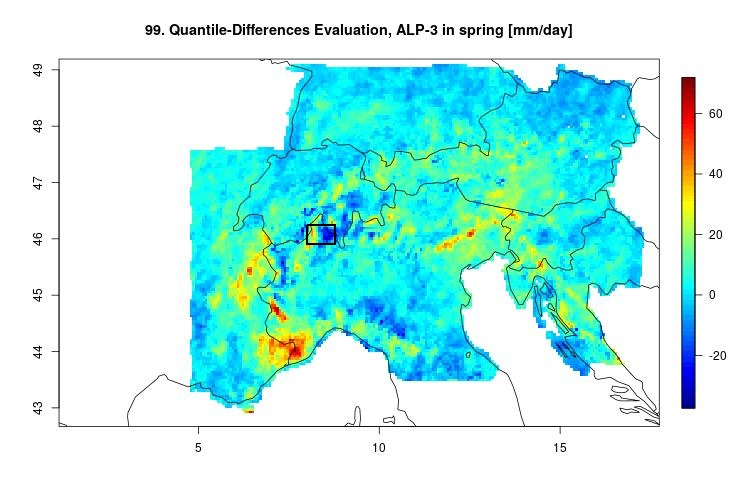
\includegraphics[width=\textwidth]{quantile_season/eval_alp3_cropped_spring.jpg}
		\caption{Niederschlagskarte}
		\label{fig:seasons:cropped eval_alp_3}
	\end{subfigure}
	\begin{subfigure}{0.49\textwidth}
		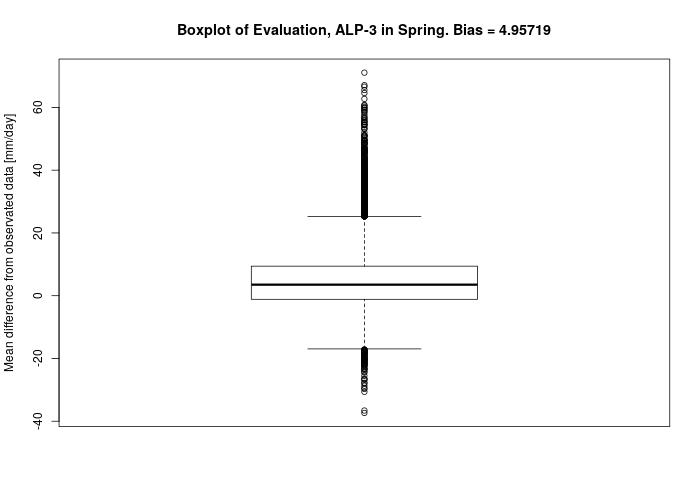
\includegraphics[width=\textwidth]{quantile_season/boxplot_eval_alp3_cropped_spring.jpg}
		\caption{Boxplot}
		\label{fig:seasons:cropped eval_alp_3_boxplot}
	\end{subfigure}
	\caption{Differenzen des Niederschlags im Datensatz Evaluation ALP-3 ohne dem Gebiet im Süden Kroatiens im Frühling, mit dem gekennzeichnetem Gebiet}
\end{figure}

\begin{figure}[h!]
	\begin{subfigure}{0.49\textwidth}
		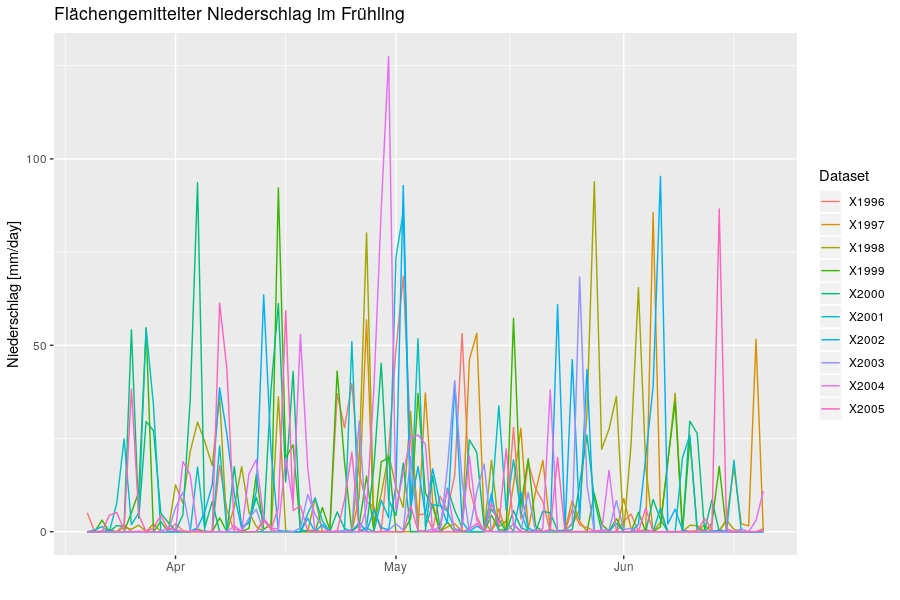
\includegraphics[width=\textwidth]{quantile_season/eval_alp3_undersim_frequencies.jpeg}
		\caption{Flächengemittelter Niederschlag in dem Bereich der Überschätzung (vgl. Abb.\ref{fig:seasons:cropped eval_alp_3} für den Datensatze Evaluation ALP-3}
		\label{fig:seasons:oversim eval_alp_3}
	\end{subfigure}
	\begin{subfigure}{0.49\textwidth}
		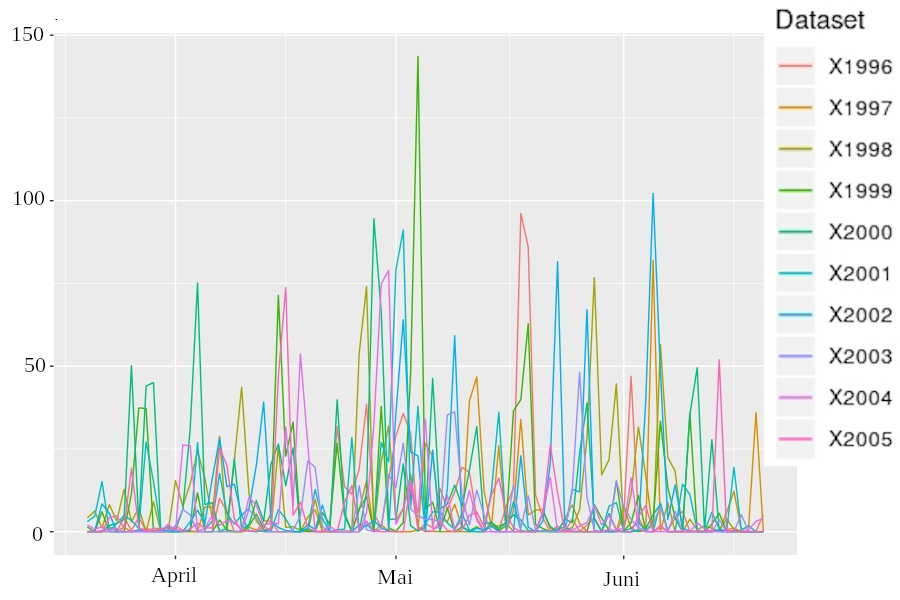
\includegraphics[width=\textwidth]{quantile_season/eval_alp3_oversim_frequencies.jpeg}
		\caption{Flächengemittelter Niederschlag in dem Bereich der Unterschätzung (vgl. Abb.\ref{fig:seasons:cropped eval_alp_3} für den Datensatze Evaluation ALP-3}
		\label{fig:seasons:undersim_eval_alp_3}
	\end{subfigure}
	\caption{}
	\label{fig:seasons:overunder_eval_alp3}
\end{figure}
\begin{figure}[h!]
	\begin{subfigure}{0.49\textwidth}
		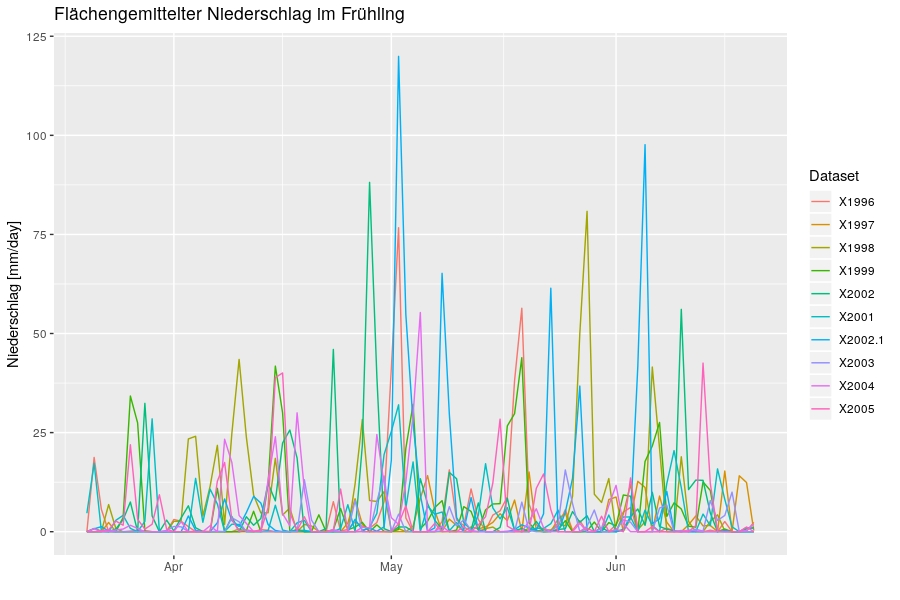
\includegraphics[width=\textwidth]{quantile_season/apgd_oversim_eval_alp3_freq.jpeg}
		\caption{Flächengemittelter Niederschlag in dem Bereich der Überschätzung (vgl. Abb.\ref{fig:seasons:cropped eval_alp_3} für die Beobachtungsdaten}
		\label{fig:seasons:oversim eval_alp_3_obs}
	\end{subfigure}
	\begin{subfigure}{0.49\textwidth}
		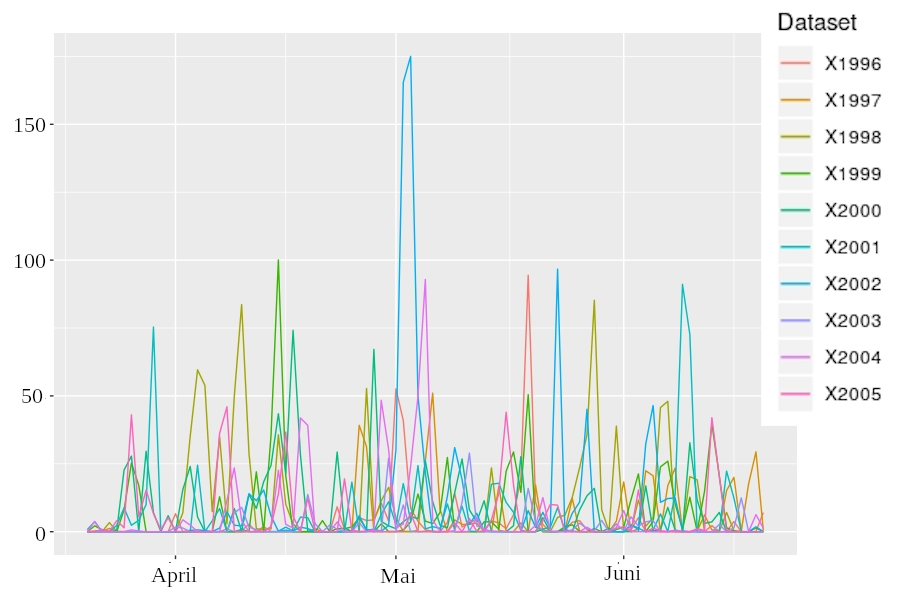
\includegraphics[width=\textwidth]{quantile_season/apgd_undersim_eval_alp3_freq.jpeg}
		\caption{Flächengemittelter Niederschlag in dem Bereich der Unterschätzung (vgl. Abb.\ref{fig:seasons:cropped eval_alp_3}) für die Beobachtungsdaten}
		\label{fig:seasons:undersim_eval_alp_3_obs}
	\end{subfigure}
	\caption{}
	\label{fig:seasons:overunder_obs_eval_alp3}
\end{figure}

Wie beim Vergleichen der beiden Häufigkeiten des flächengemittelten Niederschlags in den Abbildungen \ref{fig:seasons:overunder_eval_alp3} und \ref{fig:seasons:overunder_eval_alp3} auffällt, scheint durch das Konvektion-Simulierende downscaling-Modell die Beobachtungsdaten besser dargestellt zu werden als das in Kapitel \ref{subsec:hist_eur11} verglichene Modell mit parametrisierter Konvektion:
\begin{itemize}
	\item Der Unterschied zwischen den größten Peaks beider Karten ist viel kleiner
	\item Die entsprechenden Peaks sind im richtigen Monat
\end{itemize}
Da im überschätzendem Bereich der größte Niederschlag seitens des Modells im Jahr 2004 vorhergesagt wird, wurde in diesem Jahr der Niederschlag relativ zum Durchschnittsniederschlag dieser Fläche aufgetragen, um einen besseren Vergleich dieses zu erhalten. Daraus ergab sich die Grafik in Abb. \ref{fig:seasons:pr_oversim_eval_alp3}.\\
Für den unterschätzenden Bereich wurden dieselben Berechnungen ausgeführt für das Jahr 2002, da dort die Beobachtungsdaten den markantesten Peak erreichen und so die Modelldaten weit übertreffen. Die Ergebnisse sind in Abb.\ref{fig:seasons:pr_undersim_eval_alp3} zu finden.\\
\begin{figure}[h!]
	\begin{subfigure}{0.49\textwidth}
		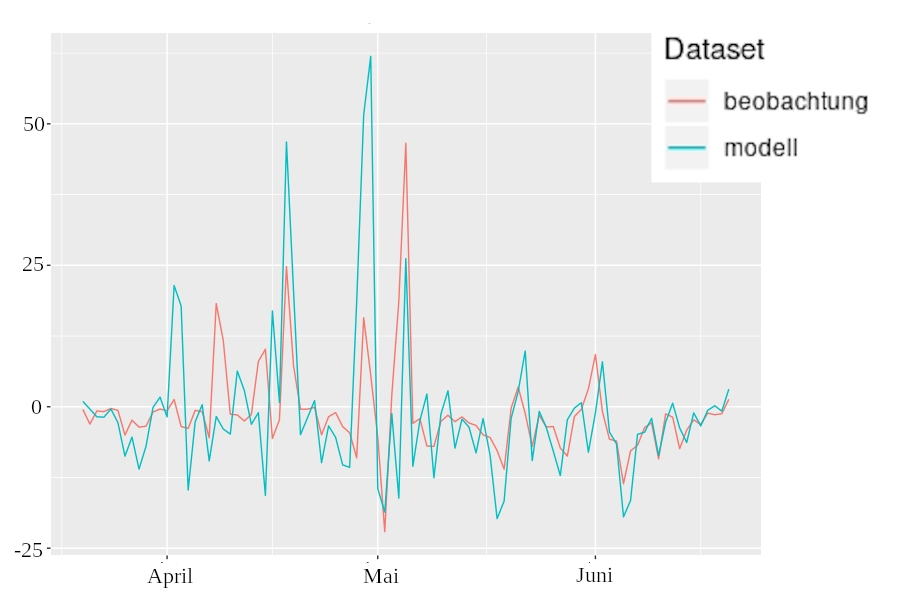
\includegraphics[width=\textwidth]{quantile_season/eval_alp3_oversim_2004.jpeg}
		\caption{Überschätzender Bereich, Jahr 2004}
		\label{fig:seasons:pr_oversim_eval_alp3}
	\end{subfigure}
	\begin{subfigure}{0.49\textwidth}
		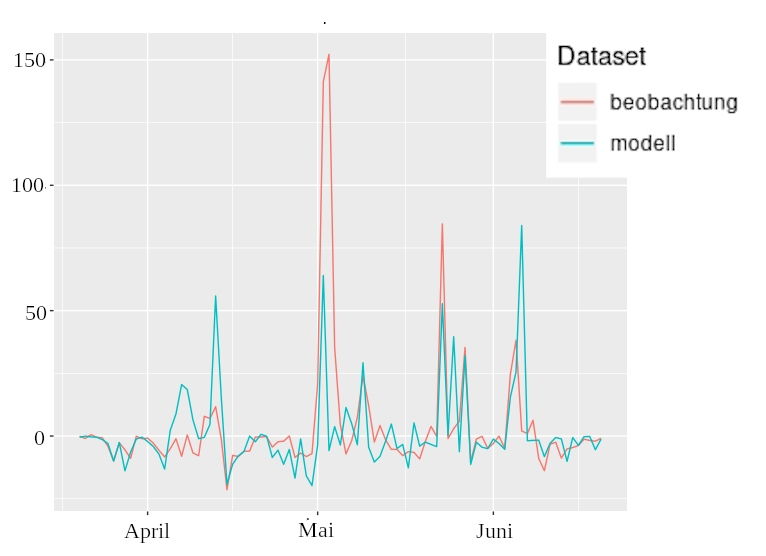
\includegraphics[width=\textwidth]{quantile_season/eval_alp3_undersim_2002.jpeg}
		\caption{Unterschätzender Bereich, Jahr 2002}
		\label{fig:seasons:pr_undersim_eval_alp3}
	\end{subfigure}
	\caption{Abweichungen vom mittleren Niederschlag im gekennzeichnetem Bereich von Abb.\ref{fig:seasons:cropped eval_alp_3}}
	\label{fig:seasons:pr_over_undersim_eval_alp3}
\end{figure}
Wie man in der Abbildung \ref{fig:seasons:pr_oversim_eval_alp3} gut erkennen kann ist der relative Niederschlag für das Jahr 2004 gut abgebildet und in der Fluktuation treffender als in der vergleichbaren Abbildung  für den Datensatz Historical EUR-11 (siehe Abb.\ref{fig:seasons:hist_eur11:oversim_mean}). Die Ausschläge scheinen zwar treffend aber zu schwach modelliert worden zu sein.\\
In der Abbildung \ref{fig:seasons:pr_undersim_eval_alp3} sind die Ausschläge für den unterschätzenden Bereich dargestellt: Man erkennt wieder, dass die Fluktuation um einiges Besser dargestellt ist, als in der vergleichbaren Darstellung vom Historical EUR-11 Datensatz. Hier scheinen die Daten das Spiegelbild des überschätzenden Bereichs zu sein: Die Ausschläge der Kurven sind Gegenläufig zueinander.

\subsection{Zusammenfassung}
Wie in den vorhergehenden Unterkapiteln gezeigt wurde, scheint das downscaling-Modell mit simulierter Konvektion die Frequenz der Fluktuationen im Niederschlag bzw. in der Temperatur den Beobachtungsdaten entsprechender darzustellen. Dies äußert sich vor allem im Niederschlag gegen den entsprechenden Durchschnitt: Der Niederschlag scheint im Modell mit parametrisierter Konvektion mit einer gegebenen Frequenz zu alternieren, ohne die Beobachtungsdaten tatsächlich abzubilden.\\
Die Temperaturkurve scheint diesem Muster zu folgen, wie in der Abb.\ref{fig:seasons:mean_alp3} zu sehen ist, ist sie im Modell CCLM5-0-9 um einiges treffender dargestellt.\\
Der größte Nachteil für den Einsatz der dynamisch simulierten Konvektion ist, dass sich durch die Simulation viele Fehlerquellen in gebirgigen Gebieten einschleichen können, wenn die Parameter noch nicht hinreichend fein-getuned wurden. Dies ist besonders gut in dem Unterkapitel \ref{subsec:hist_eur11} und \ref{subsec:eval_alp3} zu sehen. Dort wurden Abweichungen großer positiven Wertes geographisch direkt neben solchen negativen Wertes lokalisiert. Durch solche Gebiete starker Abweichung verschiebt sich in Folge auch der Bias für die Starkregenereignisse.\\
Somit kann gesagt werden, dass die dynamisch simulierte Konvektion in regionalen Klimamodellen CCLM5-0-9 zu stärkeren Ausschlägen der Abweichungen führt, auf großen Gebieten jedoch die tatsächlichen Wetterverhältnisse besser dargestellt werden als im Modell mit parametrisierter Konvektion (vgl. Abb. \ref{fig:seasons_dif}). Wird jedoch die Auswirkung eines globalen Klimamodells auf ein gebirgiges Gebiet wie die Alpen betrachtet, liefert das Klimamodell CCLM5-0-9 derzeit noch schlechtere Vorhersagen als das CCLM4-8-17, da dort die Ausschläge der Abweichungen weniger markant sind. Dieses Modell hat einen klaren Altersvorteil wodurch die Parameter feiner abgestimmt werden konnten. Somit konnte im Schnitt die Abweichung für dieses Modell heruntergesetzt werden.\\
Will man jedoch klimatische Zustände simulieren, welche dem jetzigen Zustand unähnlich sind, muss auf die explizit simulierte Konvektion zurückgegriffen werden da in der parametrisierten Konvektion nur die bisherigen Wettererscheinungen in die Berechnungen einbezogen werden und sich somit keine neuen Wettererscheinungen zeigen lassen, welche aus einer stark abweichenden atmosphärischen Konstellation resultieren würden.\\

\section{R-Code}
\begin{lstlisting}[language = R]
getQuantileOfSeasons <- function(list_all_days){
	qt_by_year<-list(spring=NULL, summer=NULL, autumn=NULL, winter=NULL)
	for(i in 1:4){
		qt_by_year[[i]]<- calc(list_all_days[[i]],Q99)
	}
	return(qt_by_year)
}
eval_eur11_seasons<-list(spring=stack(paste0(output_dir, "eval_eur11_spring.nc")), summer= stack(paste0(output_dir, "eval_eur11_summer.nc")),
autumn=stack(paste0(output_dir, 'eval_eur11_autumn.nc')), winter=stack(paste0(output_dir, 'eval_eur11_winter.nc'))) # Zuvor aufsplitten der Daten in die Jahreszeiten
eval_eur11_seasons_q99<-getQuantileOfSeasons(eval_eur11_seasons)#quantile berechnen
dif_eval_eur11<-overlay(quantile_eval_eur11, quantile_observations, fun=function(x,y){return((x - y))})# differenzen Berechnen
\end{lstlisting}

Für nähere Informationen zu den Funktionen muss auf das git-Repositorium verwiesen werden, welches im Anhang gefunden werden kann.